\documentclass{article}
\usepackage{graphicx} % Required for inserting images
\usepackage{float} 
\usepackage{amsmath,amssymb,amsfonts}
\usepackage{xspace}
\usepackage{hyperref}
\hypersetup{
%\ifpdf
%        pdftex,
%\else
%        dvipdf,
%\fi
  %pdftex,              % using ps2pdf vs pdftex
  %ps2pdf,              % using ps2pdf vs pdftex
        %hypertex,
  colorlinks=true,     % color the words instead of use a colored box
  urlcolor=blue,       % \href{...}{...} external (URL)
%  filecolor=blue,      % \href{...} local file
  linkcolor=blue,     % \ref{...} and \pageref{...}
  citecolor=blue,     % \cite{}
% letterpaper=true,
  plainpages=false,
%    plainpages          boolean         true
%    Forces page anchors to be named by the arabic form of the page number,
%    rather than the formatted form.
  breaklinks=true,
%    breaklinks          boolean         false
%    Allows link text to break across lines; since this cannot be accommodated in
%    PDF, it is only set true by default if the pdftex driver is used. This makes
%    links on multiple lines into different PDF links to the same target.
% pagebackref=true,
%     Adds ?backlink? text to the end of each item in the bibliography, as a list
%     of section numbers. This can only work properly if there is a blank line
%     after each \bibitem.
  bookmarksnumbered=true,
%    bookmarksnumbered   boolean         false
%    If Acrobat bookmarks are requested, include section numbers.
  bookmarksopen=true,
%    bookmarksopen       boolean         false
%    If Acrobat bookmarks are requested, show them with all the subtrees expanded.
  pdftitle={mariposa unsat core figures},
  pdfauthor={},
  pdfkeywords={},
% pdfpagelabels=true,
  pdfpagemode=UseOutlines  % None, UseThumbs, UseOutlines, FullScreen
}
\usepackage[margin=1in]{geometry}
\newcommand{\name}{Mariposa\xspace}

\newcommand{\bname}{Mariposa\xspace}

\newcommand{\funding}{We received money from...}
\newcommand{\unsat}{\texttt{unsat}\xspace}
\newcommand{\sat}{\texttt{sat}\xspace}
\newcommand{\timeout}{\texttt{timeout}\xspace}
\newcommand{\unknown}{\texttt{unknown}\xspace}
\newcommand{\exception}{\texttt{exception}\xspace}

\newcommand{\fstar}{F${}^\star$\xspace}

\newcommand{\dkomodo}{Komodo$_{D}$\xspace}
\newcommand{\dlvbkv}{VeriBetrKV$_{L}$\xspace}
\newcommand{\dfvbkv}{VeriBetrKV$_{D}$\xspace}
\newcommand{\fsdice}{DICE$^\star_F$\xspace}
\newcommand{\fsvwasm}{vWasm$_F$\xspace}
\newcommand{\skomodo}{Komodo$_S$\xspace}

\newcommand{\shuffle}{\textbf{shuffling}\xspace}
\newcommand{\rename}{\textbf{renaming}\xspace}
\newcommand{\reseed}{\textbf{reseeding}\xspace}

\newcommand{\unsolvable}{\texttt{unsolvable}\xspace}
\newcommand{\stable}{\texttt{stable}\xspace}
\newcommand{\unstable}{\texttt{unstable}\xspace}
\newcommand{\inconclusive}{\texttt{inconclusive}\xspace}
\begin{document}

\subsection{\unsat core experiment results summary (placeholder name)}

\begin{figure}[H]
    \begin{minipage}[c]{\textwidth}
      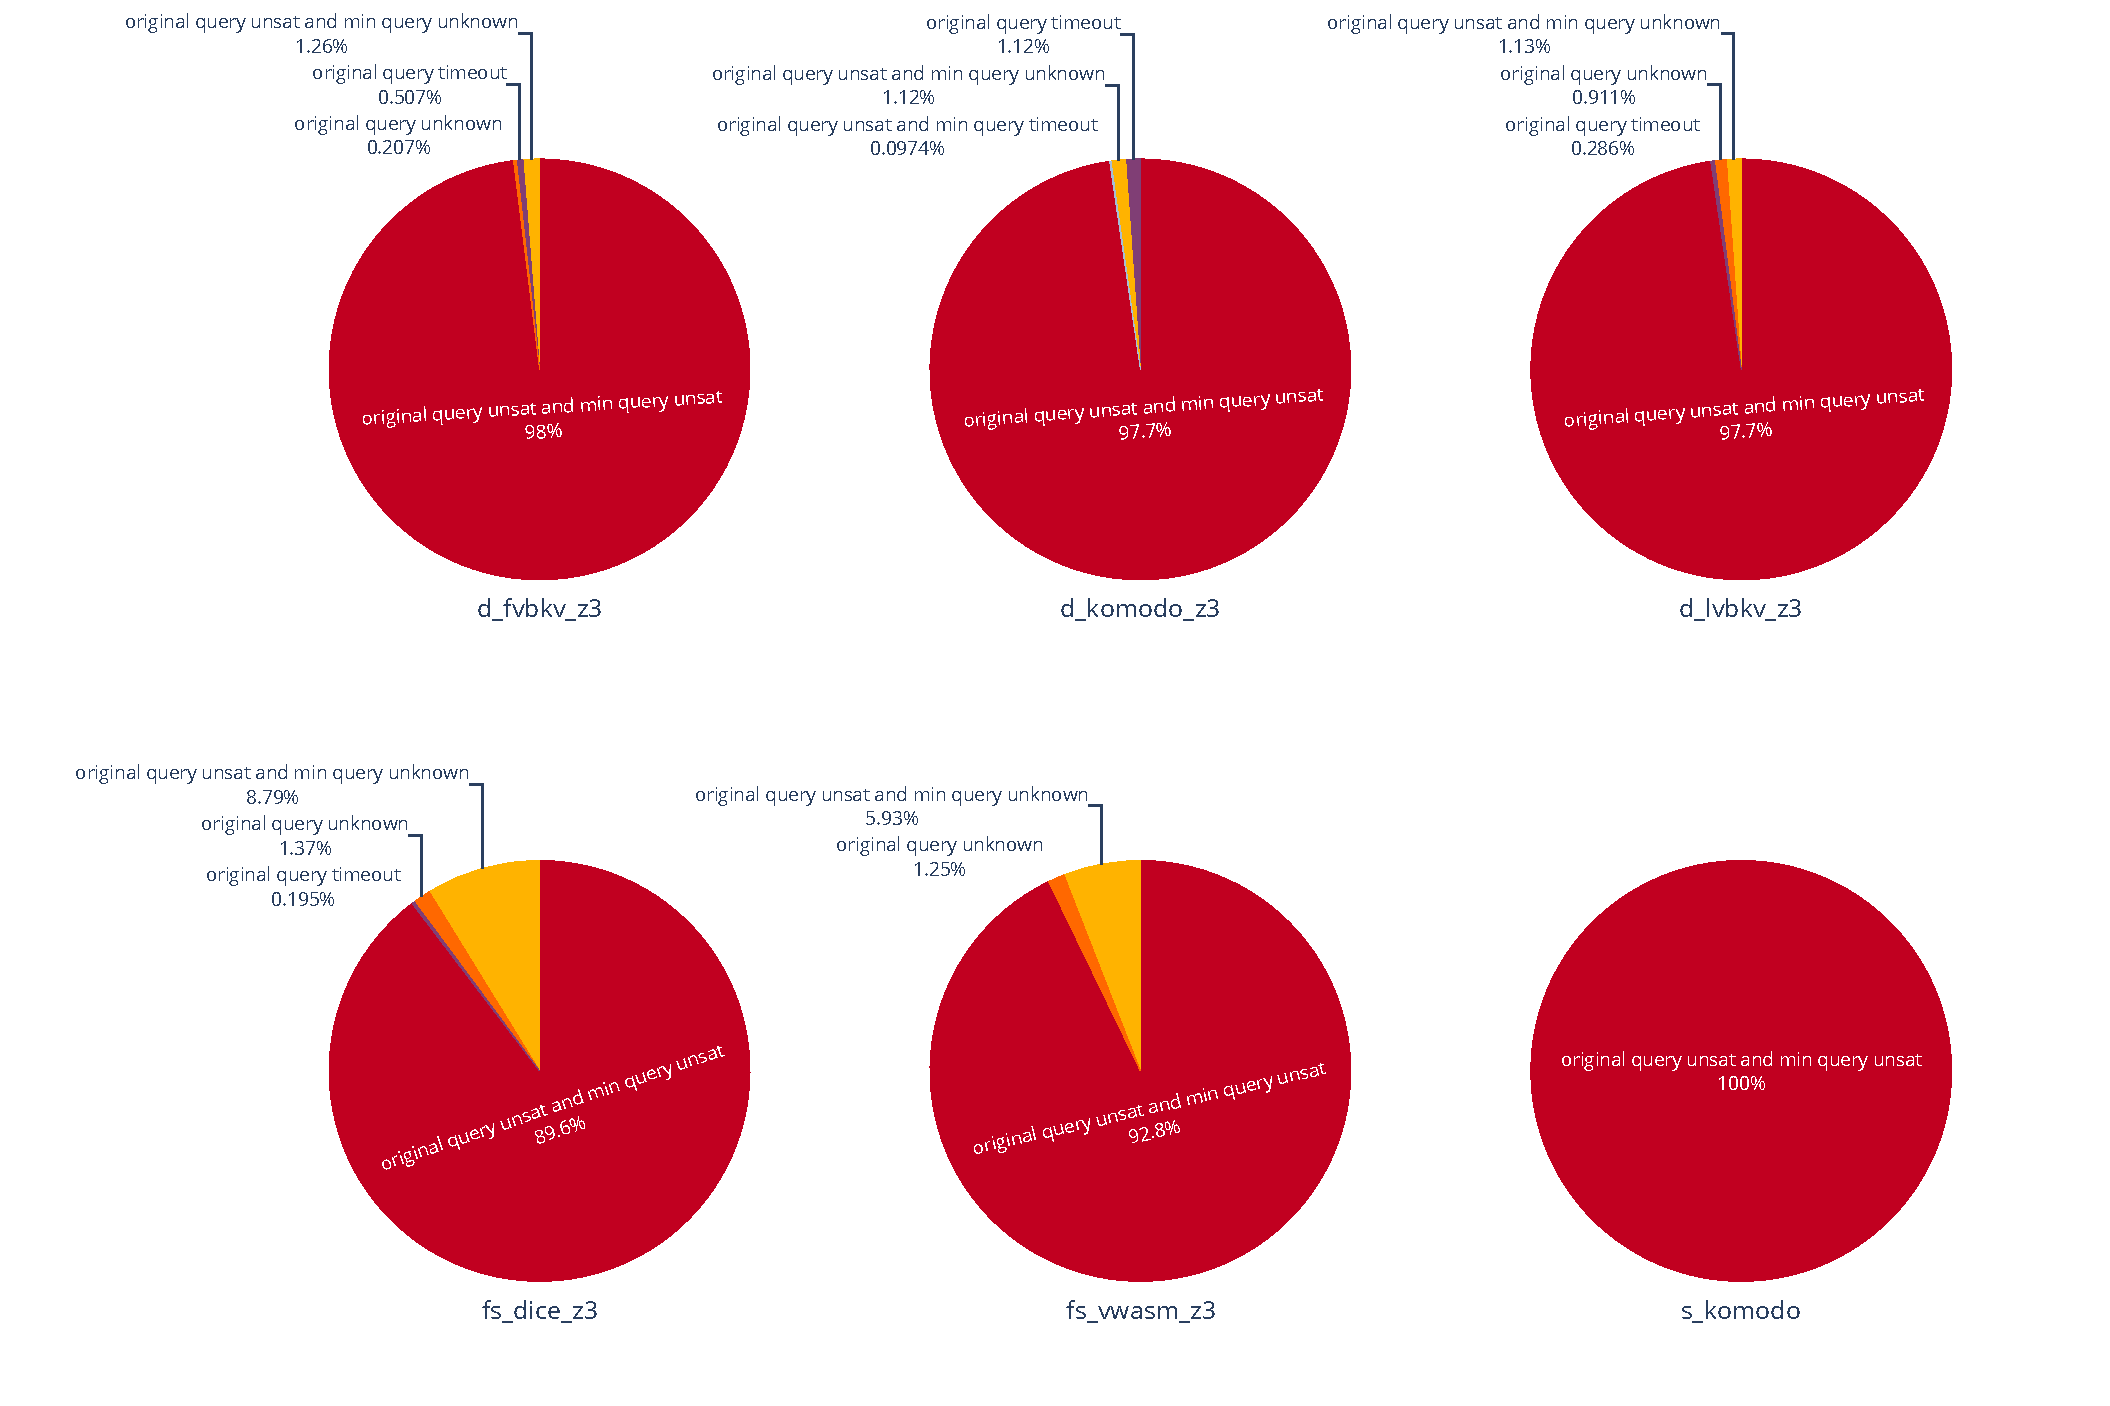
\includegraphics[width=\textwidth]{figs/unsat_core/all_pie_plotly.pdf}
      \vspace{-0.5cm}
      \caption{\textbf{Query result proportions.} Queries from each project were divided into 5 categories: original query \timeout, original query \unknown, original query \unsat and min query \timeout, original query \unsat and min query \unknown, original query \unsat and min query \unsat. Min (minimized asserts) queries were created from original queries that returned an \unsat core, which is only possible if the original query returns \unsat. Note that projects from the same language had similar proportions of original query \unsat and min query \unsat.
      }
      \label{fig:dkomodo_pert_ext}
      \vspace{0.5cm}
    \end{minipage}
\end{figure}

\clearpage

\subsection{Runtime and filesize \unsat core changes (placeholder name)}
\begin{figure}[H]
    \begin{minipage}[c]{\textwidth}
      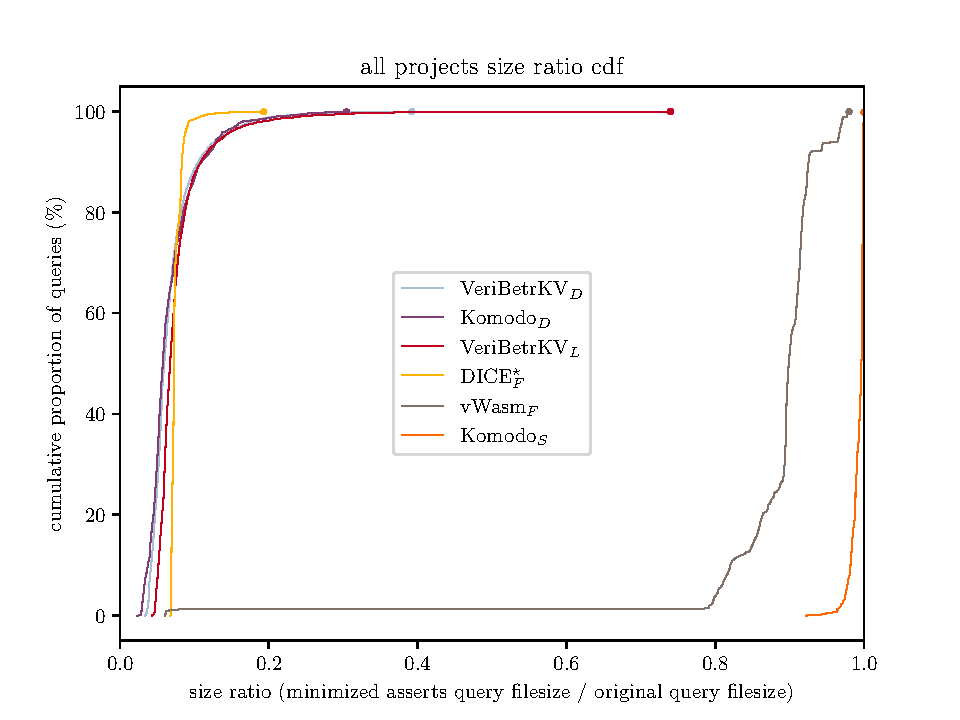
\includegraphics[width=\textwidth]{figs/unsat_core/all_size.pdf}
      \vspace{-0.5cm}
      \caption{\textbf{Size ratio after keeping only the \unsat core.} File size ratios were calculated for pairs of original and corresponding minimized asserts queries where the original query returned an \unsat core and plotted on a CDF. It appears that the queries of Dafny projects and \fsdice tend to contain many asserts that are unessential to the `\unsat' result. On the other hand, \fsvwasm and \skomodo's queries tend to contain a higher proportion of asserts important to the `\unsat' result.}
      \label{fig:unsat_core_all_size}
      \vspace{0.5cm}
    \end{minipage}
\end{figure}

\clearpage

\begin{figure}[H]
    \begin{minipage}[c]{\textwidth}
      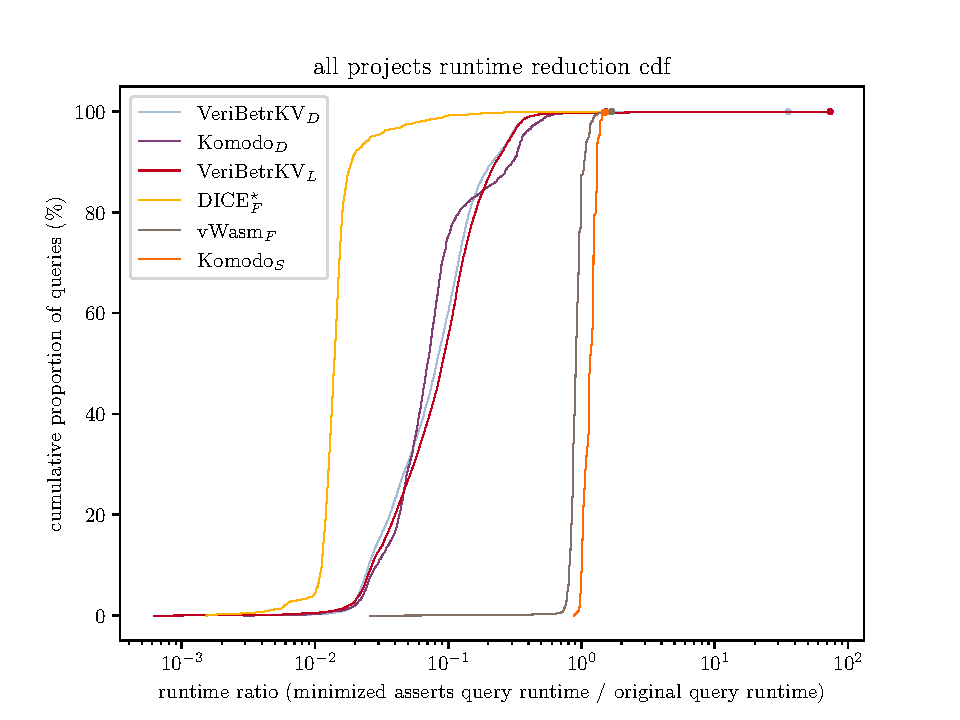
\includegraphics[width=\textwidth]{figs/unsat_core/all_time.pdf}
      \vspace{-0.5cm}
      \caption{\textbf{Runtime comparison between original and minimized asserts queries.} Runtime ratios were calculated for pairs of original and corresponding minimized asserts queries where both queries returned ‘\unsat.’ The general shape suggests that queries that consist of only asserts that make up the \unsat core typically run faster than those that do not. Notably, the most minimized queries of Dafny projects and \fsdice experienced a substantial speed up, while \fsvwasm and \skomodo minimized queries did not experience as much of a change in runtime. Unexpectedly, \dlvbkv and \dfvbkv had outliers where the minimized asserts queries took much longer (35x, 70x) than the original queries.}
      \label{fig:unsat_core_all_time}
      \vspace{0.5cm}
    \end{minipage}
\end{figure}

\clearpage

\begin{figure}[H]
    \begin{minipage}[c]{\textwidth}
      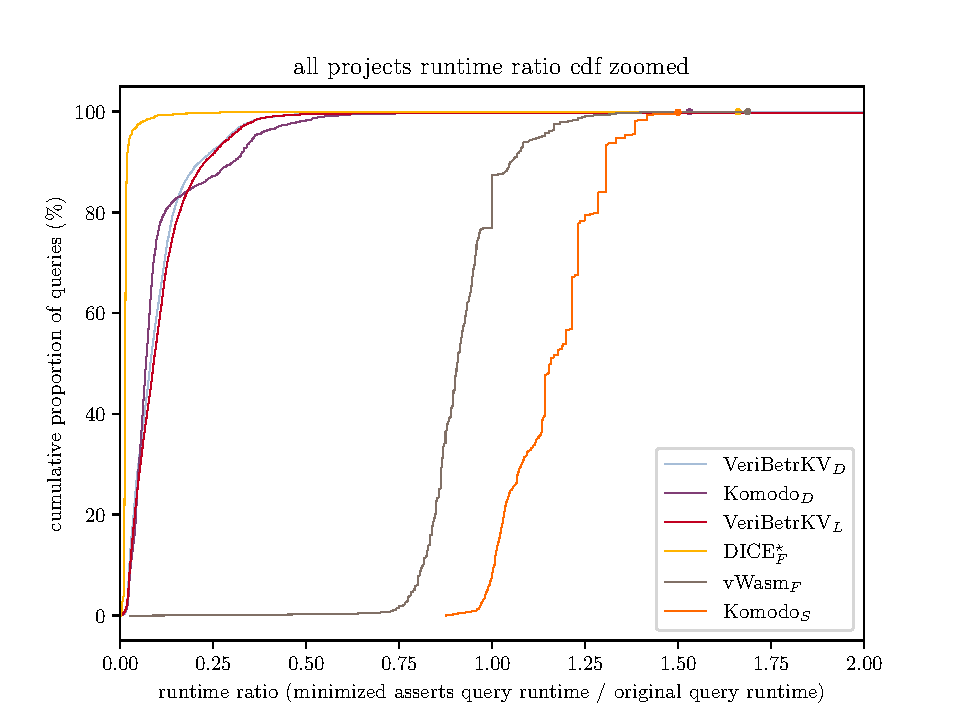
\includegraphics[width=\textwidth]{figs/unsat_core/all_time_zoomed.pdf}
      \vspace{-0.5cm}
      \caption{\textbf{Runtime comparison between original and minimized asserts queries -- zoomed.} We show the same results from figure \ref{fig:unsat_core_all_time}, but focused on the 0.00-2.00 region. We observe similarities between this figure and the file size reduction figure where Dafny projects + \fsdice saw a relative decrease in their statistics, while \fsvwasm and \skomodo did not, as well as similarities between the graphs' shapes. From this figure, it is clearer that a larger proportion of \fsvwasm and \skomodo's minimized queries take longer than the original queries.}
      \label{fig:unsat_core_all_time_zoomed}
      \vspace{0.5cm}
    \end{minipage}
\end{figure}

\clearpage

\subsection{Placeholder subsection title}
\begin{figure}[H]
    \begin{minipage}[c]{\textwidth}
      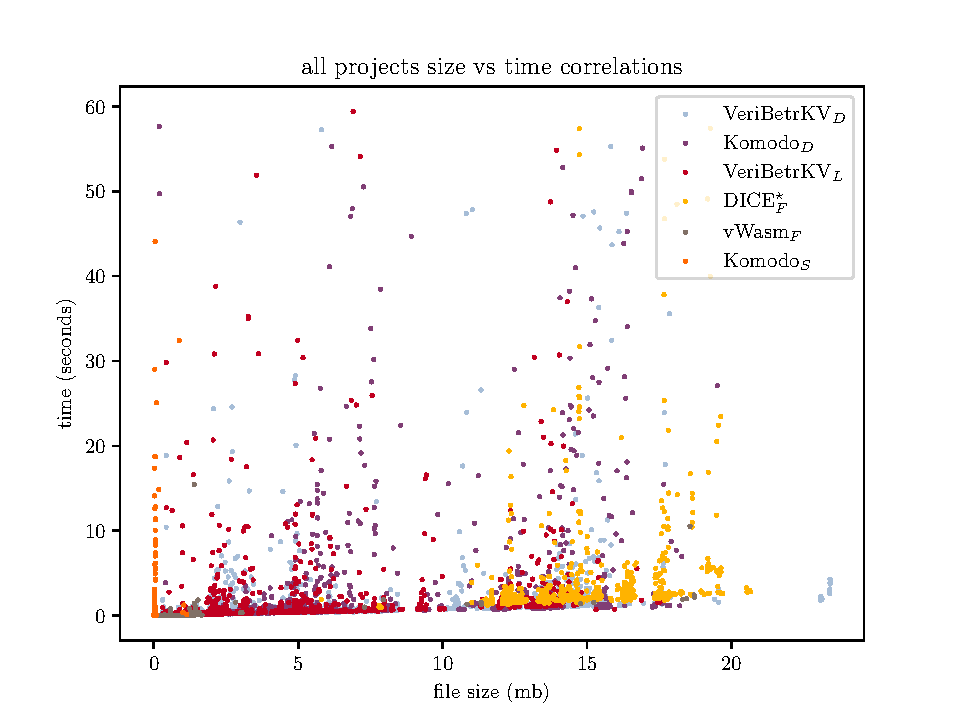
\includegraphics[width=\textwidth]{figs/unsat_core/size_vs_time.pdf}
      \vspace{-0.5cm}
      \caption{\textbf{Size vs time graph} We plot file size (MB) vs time (sec) for each original query that returned `\unsat' on version 4.8.5. A linear lower bound is visible on the graph. Most queries fall close to this lower bound (3-4 seconds within) but there is a substantial number of outliers.}
      \label{fig:dkomodo_pert_ext}
      \vspace{0.5cm}
    \end{minipage}
\end{figure}

\clearpage


\end{document}



